\documentclass[a4paper,oneside,12pt]{article}

\usepackage[slovene]{babel}    % slovenian language and hyphenation
\usepackage[utf8]{inputenc}    % make čšž work on input
\usepackage[T1]{fontenc}       % make čšž work on output
\usepackage[reqno]{amsmath}    % basic ams math environments and symbols
\usepackage{amssymb,amsthm}    % ams symbols and theorems
\usepackage{mathtools}         % extends ams with arrows and stuff
\usepackage{url}               % \url and \href for links
\usepackage{icomma}            % make comma a thousands separator with correct spacing
\usepackage{units}             % \unit[1]{m} and unitfrac
\usepackage{enumerate}         % enumerate style
\usepackage{array}             % mutirow
\usepackage[usenames]{color}   % colors with names
\usepackage{graphicx}          % images

\usepackage[bookmarks, colorlinks=true, linkcolor=black, anchorcolor=black,
  citecolor=black, filecolor=black, menucolor=black, runcolor=black,
  urlcolor=black, pdfencoding=unicode]{hyperref}  % clickable references, pdf toc
\usepackage[
  paper=a4paper,
  top=2.5cm,
  bottom=2.5cm,
  textwidth=15cm,
% textheight=24cm,
]{geometry}  % page geomerty

\newtheorem{izrek}{Izrek}
\newtheorem{posledica}{Posledica}

\theoremstyle{definition}
\newtheorem{definicija}{Definicija}
\newtheorem{opomba}{Opomba}
\newtheorem{zgled}{Zgled}

% basic sets
\newcommand{\R}{\ensuremath{\mathbb{R}}}
\newcommand{\N}{\ensuremath{\mathbb{N}}}
\newcommand{\Z}{\ensuremath{\mathbb{Z}}}
\renewcommand{\C}{\ensuremath{\mathbb{C}}}
\newcommand{\Q}{\ensuremath{\mathbb{Q}}}

% greek letters
\let\oldphi\phi
\let\oldtheta\theta
\newcommand{\eps}{\varepsilon}
\renewcommand{\psi}{\varpsi}
\renewcommand{\theta}{\vartheta}

% vektorska analiza
\newcommand{\grad}{\operatorname{grad}}
\newcommand{\rot}{\operatorname{rot}}
\renewcommand{\div}{\operatorname{div}}

% lists with less vertical space
\newenvironment{itemize*}{\vspace{-6pt}\begin{itemize}\setlength{\itemsep}{0pt}\setlength{\parskip}{2pt}}{\end{itemize}}
\newenvironment{enumerate*}{\vspace{-6pt}\begin{enumerate}\setlength{\itemsep}{0pt}\setlength{\parskip}{2pt}}{\end{enumerate}}
\newenvironment{description*}{\vspace{-6pt}\begin{description}\setlength{\itemsep}{0pt}\setlength{\parskip}{2pt}}{\end{description}}

\newcommand{\Title}{}
\newcommand{\Author}{Jure Slak}
\title{\Title}
\author{\Author}
\date{\today}
\hypersetup{pdftitle={\Title}, pdfauthor={\Author}, pdfcreator={\Author},
            pdfproducer={\Author}, pdfsubject={}, pdfkeywords={}}  % setup pdf metadata

% \pagestyle{empty}              % vse strani prazne
% \setlength{\parindent}{0pt}    % zamik vsakega odstavka
% \setlength{\parskip}{10pt}     % prazen prostor po odstavku
\setlength{\overfullrule}{30pt}  % oznaci predlogo vrstico z veliko črnine

\begin{document}

\noindent \parbox{9cm}{
  {\bf \v{S}tudentski svet FMF
    Jadranska 19\\
    1000 Ljubljana
  }}
  \hfill\parbox{5.5cm}
  {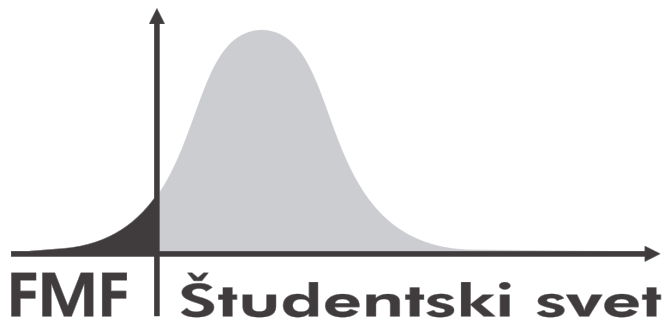
\includegraphics[scale=0.7]{Slyka}
  }

\vspace{20pt}

\section*{Uradno mnenje ŠS FMF glede \\ elektronskega sporočila doc. Kobala}

V zadnjem tednu se je v medijih pojavila zgodba doc. Kobala, ki je študentom, ki jim je kljub prepozno oddani prošnji za vpis le-to odobril, poslal sporno elektronsko sporočilo.

V ŠS FMF smo v začetku šolskega leta dobili anonimno sporočilo, v katerem nam je študent poslal tudi besedilo spornega sporočila in s tem želel opozoriti, na neprimerno obnašanje doc. Kobala ter zagotoviti, da se kaj takega ne ponovi. Ocenili smo, da je bilo besedilo res neprimerno in se o njem pogovorili tudi s predstojnico oddelka za matematiko. Zagotovila nam je, da bo doc. Kobala opozorila na neustreznost vsebine in da se kaj podobnega v prihodnosti ne bo več zgodilo, saj med drugim doc. Kobal ni več na tej funkciji.

V ŠS FMF se nam sporočilo ni zdelo primerno, vendar pa je treba kot v vseh podobnih primerih vedno oceniti celotno situacijo, ne le vzeti nekaj vrstic iz konteksta. Kljub nerodno napisanemu sporočilu, povezav med njim in dobrodelno organizacijo ni, namen obiska predavanja (in morebitne donacije) pa je bila le nekakšna neformalna kazen zamudnikom po tem, ko je bilo njihovi prošnji že ugodeno, z namenom vzgoje in da bi preprečili ponavljanje takega obnašanja. Šlo je namreč za posameznike, ki so prošnje oddali prepozno in tako formalno gledano niso ustrezali pogojem za vpis. Marsikje bi njihove prošnje v izogib različnim težavam takoj zavrnili oz. jih sploh ne bi obravnavali. Doc. Kobal se je kljub temu odločil za obravnavo, saj se mu za le nekaj dni zamujen rok ni zdela tako velika napaka, da bi si študentje zaslužili vse težave, ki pridejo z izgubo študentskega statusa. To je bil zelo človeški in korekten pristop, ki ga študentje na naši fakulteti zelo cenimo.

Zaradi objave članka v medijih je ŠS FMF študentom, ki so mail prejeli, poslal poziv, da se odzovejo na objavo v
medijih. Študentje, ki so se javili pozivu, so potrdili, da so sporočilo razumeli kot vzgojno in dobronamerno in v njem niso videli nič spornega. V trenutku ko so mail prejeli, so bili namreč že vpisani v letnik in so vedeli, da udeležba ali donacija nikakor nista bili pogoj za karkoli. Tudi v ŠS FMF se strinjamo, da z opozarjanjem študentov na to, da njihove zamude lahko povročijo veliko težav, ni nič narobe.

V ŠS FMF menimo, da je doc. Kobal šel predaleč in se obnašal neprofesionalno, saj vsebina maila, sploh omenjanje donacij za društvo, predstavljeno na seminarju, ki ga organizira sam, ni bila primerna, vendar vseeno ocenjujemo, da ni šlo za tako sporno dejanje, kot je na prvi pogled razvidno iz zgodbe v Delu. \\

\noindent V imenu SŠ FMF, \\
Marion van Midden \hfill Ljubljana, \today

% text here

\end{document}
% vim: syntax=tex
% vim: spell spelllang=sl
% vim: foldlevel=99
% Latex template: Jure Slak, jure.slak@gmail.com

